    \chapter{Solution of Nonlinear Equations}
    
    \subsection*{Applications}
    \begin{itemize}
        \item Intersection / collision detection
        \item Optimization (we'll see the connection later)
    \end{itemize}
    
    \section{Bisection}
    \begin{figure}
      \centering
      \begin{subfigure}[b]{0.3\textwidth}
        \resizebox{\textwidth}{!}{
          \begin{tikzpicture}
\begin{axis}[
axis y line=center,
axis x line=middle,
scale only axis,
axis equal,
xmax=3,xmin=-3,
ymin=-4,ymax=4,
ticks=none,
width=5cm,
samples=100,
anchor=center,
]
\addplot[thick,domain=-5:0.9,mark=none]{-0.2*x/(1-x) -1};
\addplot[thick,domain=1.1:5,mark=none]{-x/(1-x) -1};
\addplot[thick,mark=none,dashed] coordinates {(1, -4) (1, 4)};
% \addplot[thick,mark=none,dashed] {-1};
\end{axis}
\end{tikzpicture}

        }
        \caption{Singularities}
      \end{subfigure}
      \begin{subfigure}[b]{0.3\textwidth}
        \resizebox{\textwidth}{!}{
          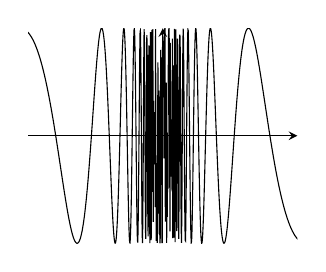
\begin{tikzpicture}
\begin{axis}[
axis y line=center,
axis x line=middle,
xmax=0.2,xmin=-0.2,
ymin=-1,ymax=1,
ticks=none,
width=5cm,
anchor=center,
]
\addplot [domain=-0.5:0.5,samples=2000] {sin(deg(1/x))};
\end{axis}
\end{tikzpicture}

        }
        \caption{Many Roots}
      \end{subfigure}
      \begin{subfigure}[b]{0.3\textwidth}
        \resizebox{\textwidth}{!}{
          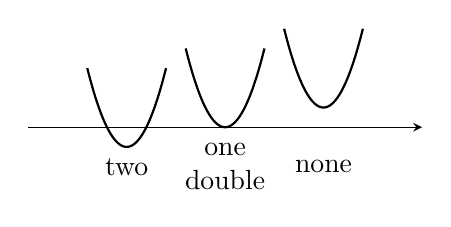
\begin{tikzpicture}
\begin{axis}[
axis y line=none,
axis x line=middle,
scale only axis,
axis equal,
ymin=-1,ymax=1,
xmin=-10,xmax=10,
ticks=none,
width=5cm,
samples=100,
anchor=center,
]
\addplot[thick,domain=-7:-3,mark=none]{(x+5)^2-1};
\addplot[thick,domain=-2:2,mark=none]{(x)^2};
\addplot[thick,domain=3:7,mark=none]{(x-5)^2+1};

\node[align=center] at (axis cs:0,-2) {one\\double};
\node at (axis cs:-5,-2) {two};
\node at (axis cs:5,-2) {none};
\end{axis}
\end{tikzpicture}

        }
        \caption{Double Roots}
      \end{subfigure}
      \label{fig:difficult-root-finding}
    \end{figure}

    \begin{figure}
      \centering
      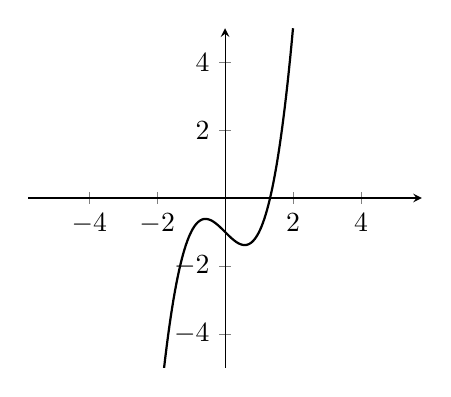
\begin{tikzpicture}
\begin{axis}[
axis y line=center,
axis x line=middle,
scale only axis,
axis equal,
xmax=2,xmin=-2,
ymin=-5,ymax=5,
width=5cm,
samples=100,
anchor=center,
]
\addplot[thick,domain=-2:2,mark=none]{x^3-x-1};
\end{axis}
\end{tikzpicture}

      \label{fig:bisection_example}
    \end{figure}

    
    \section{Regula Falsi}
    \begin{figure}
      \centering
      \begin{tikzpicture}[scale=2]
  \tkzInit[
    xmin=-3.5,xmax=1.5,
    ymin=-3,ymax=3
  ]
  \tkzFct[domain=-3:1]{exp(\x)-1}
  \tkzDefPointByFct(1) \tkzGetPoint{B} 
  \tkzDefPointByFct(-3) \tkzGetPoint{A} 
  \tkzDefPointByFct(-1) \tkzGetPoint{F} 
  \tkzDefPoint(-3.5,0){X'}
  \tkzDefPoint(0,0){O}
  \tkzDefPoint(1.5,0){X}
  \tkzDefPointBy[projection=onto O--X](A) \tkzGetPoint{A'}
  \tkzDefPointBy[projection=onto O--X](B) \tkzGetPoint{B'}
  \tkzDrawSegment[dashed](A,B)
  \tkzInterLL(A,B)(O,X) \tkzGetPoint{w}
  \tkzDrawSegment[dashed](A,A')
  \tkzLabelSegment(A,A'){$a_n$}
  \tkzDrawSegment[dashed](B,B')
  \tkzDrawSegment[->](X',X)
  \tkzLabelSegment(B,B'){$b_n$}
  \tkzLabelPoint(A){$(a_n,f(a_n))$}
  \tkzLabelPoint(B){$(b_n,f(b_n))$}
  \tkzLabelPoint(w){$w$}
  \tkzLabelPoint(X){$x$}
  \tkzDrawPoints(A,B,O,w,A',B')
  \node[pin=330:{actual root}] at (O){};
  \node[pin=120:{new estimate}] at (w){};
  \node[pin=330:{$f(x)$}] at (F){};
\end{tikzpicture}

    \end{figure}
    \begin{figure}
      \centering
      \begin{tikzpicture}[scale=2]
  \tkzInit[
    xmin=-3.5,xmax=1.5,
    ymin=-3,ymax=3
  ]
  \tkzFct[domain=-3:1]{exp(\x)-1}
  \tkzDefPointByFct(1) \tkzGetPoint{B} 
  \tkzDefPointByFct(-3) \tkzGetPoint{A} 
  \tkzDefPoint(-3.5,0){X'}
  \tkzDefPoint(0,0){O}
  \tkzDefPoint(1.5,0){X}
  \tkzDrawSegment[->](X',X)
  \tkzLabelPoint[above](X){$x$}
  \foreach \i in {0,...,2}
  {
    \tkzDrawSegment[dashed](A,B)
    \tkzInterLL(A,B)(O,X) \tkzGetPoint{W}
    \tkzDefPointBy[projection=onto O--X](A) \tkzGetPoint{A'}
    \tkzDrawSegment[dashed](A,A')
    \tkzGetPointCoord(W){w}
    \tkzDefPointByFct(\wx) \tkzGetPoint{A}
    \tkzLabelPoint(A'){$a_\i$}
  }

    \tkzDefPointBy[projection=onto O--X](B) \tkzGetPoint{B'}
  \tkzDrawSegment[dashed](B,B')
  \tkzLabelPoint(B'){$b_0, b_1, b_2, b_3$}
  \tkzDrawPoints(O)
  \tkzLabelPoint(O){root}
\end{tikzpicture}

    \end{figure}
    \begin{figure}
      \centering
      \input{figures/chap_04/04-two-sided-convergence-convex.tikz}
    \end{figure}
    
    \subsection{Termination Conditions}
    
    \section{Secant Method}
    
    \section{Newton's Method (Newton-Raphson)}
    
    \section{Inverse Quadratic Interpolation}
    
    \section{Rates of Convergence}
    
    \subsection{Newton's Method - Quadratic Convergence}
    
    \subsection{Secant Method}
    
    \section{Systems of Equations - Higher-dimensional Zeroes}
